\subsection{Неэквидистантные антенные решётки и неравномерные амплитудные распределения}\label{sect:distributions-theory}


Классическим подходом к оптимизации антенных решёток является применение различных амплитудных и геометрических
распределений \cite{harrington1961sidelobe, ma1963note, brown1962note}.Под оптимизацией понимается уменьшение
количества антенных элементов при сохранении заданнойширины главного лепестка и поддержания низкого уровня
боковых и дифракционных лепестков диаграммы направленности, либо улучшение
характеристик ДНА при том же либо меньшем количестве элементов.
Целью методов, которые применяют такой подход является нахождение таких амплитудных распределений и положений
антенных элементов при которых будут достигнуты наилучшие характеристики диаграммы направленности при
заданном максимальном количестве каналов антенной решётки. Методы этой группы включают в себя ручную
оптимизацию на основе изначально выбранного распределения \cite{lyalin2019, kuzmin2019ring, andreasen1962linear};
поиск математических приближений \cite{ishimaru1962theory, harrington1961sidelobe};
применение итеративных функций поиска (LMS алгоритм)\cite{ma1997weighted} и вероятностных методов,
таких как генетические деревья, муравьиный алгоритм, метод роя частиц и другие.
\cite{jain2012solving, dubey2023cosecant, luo2015synthesis}.

\subsubsection{Ручная оптимизация}\label{sec:manual-optimization}

Одним из применяемых подходов заключается в выборе изначального распределения и дальнейшее его изменение
на основе некоторых гипотез о влиянии тех или иных изменений на итоговую диаграмму и в
соответствии с результатами проведённого моделирования.

В качестве примера можно привести работы \cite{lyalin2019, kuzmin2019ring}, в которых в качестве
изначального распределения выбрана кольцевая концентрическая антенная решётка, в которой элементы
расположены группами прямоугольных элементов, которые в свою очередь расположены на нескольких
концентрических кольцах. Меняя угол поворота прямоугольных групп, а также смещая по фазе концентрические
окружности, можно найти некоторое расположение, удовлетворяющее техническому заданию.
Результат такой оптимизации показан на Рисунках \ref{fig:manual-opt-pos}, \ref{fig:manual-opt-radiation-pattern}.
Видно, что уровень боковых лепестков соответствует эквидистантной решётке, а уровень
дифракционных лепестков не превышает УБЛ. При этом число антенных элементов
значительно меньше чем в эквидистантной решётке с межэлементным расстоянием $d \leq \lambda/2$ и полным заполнением апертуры.

\begin{figure}[H]
    \centering
    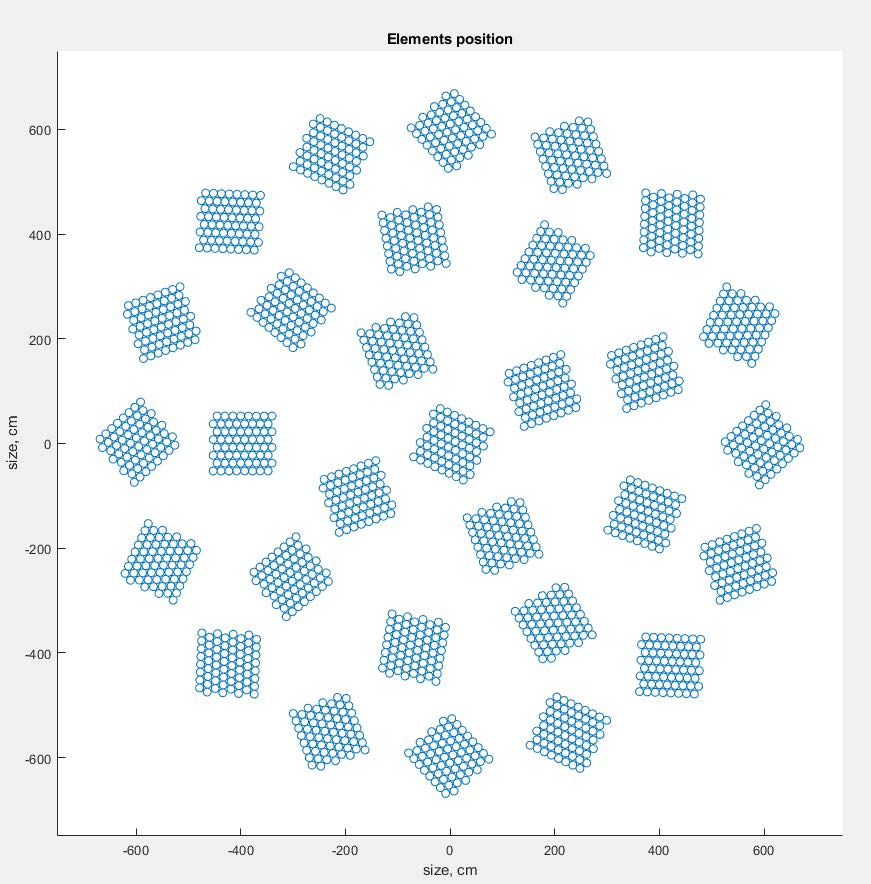
\includegraphics[width=0.8\textwidth,height=0.35\textheight,keepaspectratio]{manual-opt-pos}
    \caption{Итоговое расположение элементов}%
    \label{fig:manual-opt-pos}
\end{figure}


\begin{figure}[H]
    \centering
    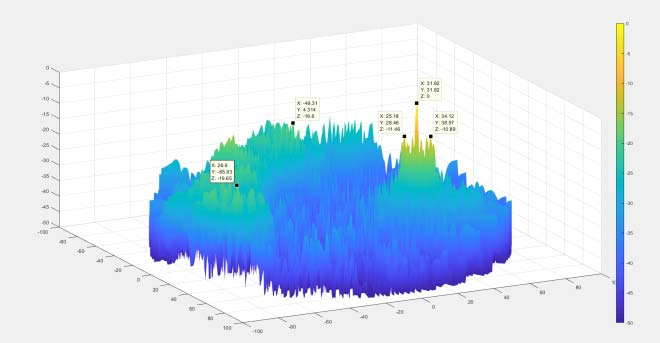
\includegraphics[width=0.8\textwidth,height=0.35\textheight,keepaspectratio]{manual-opt-radiation-pattern}
    \caption{Диаграмма направленности с отклонением на 30 градусов по углам~$\theta$~и~$\phi$. УБЛ~-11~дБ, УДЛ~-19~$\div$~-12~дБ}%
    \label{fig:manual-opt-radiation-pattern}
\end{figure}


\subsubsection{Неравномерные амплитудные распределения}\label{sect:amplitude-distributions}

Известно, что спадающие к краям амплитудные распределения позволяют уменьшить уровень боковых
лепестков при некотором расширении главного лепестка \cite{schelkunoff1943mathematical}.
Например, в работе \cite{schelkunoff1943mathematical} показно уменьшение уровня боковых
лепестков относительно решётки с равноамплитудным распределением при
использовании равномерно спадающей к краям амплитуды.

\begin{figure}[H]
    \centering
    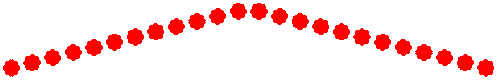
\includegraphics[width=0.8\textwidth,height=0.35\textheight,keepaspectratio]{linear-decreasing-distribution}
    \caption{Пример равномерно спадающего к краям амплитудного распределения}%
    \label{fig:linear-decreasing-distribution}
\end{figure}

Позже были рассмотрены и другие распределения похожего вида. Так, распределение вида “косинус на пьедестале”
(Рисунок~\ref{fig:partial-sum-method}), выводимое с помощью метода парциальных ДН, позволяет
проводить расчёт усилений в каналах антенной решётки по некоторым заданным характеристикам
диаграммы направленности. \cite{Chist2012}

\begin{figure}[H]
    \centering
    \begin{subfigure}[b]{0.4\textwidth}
        \centering
        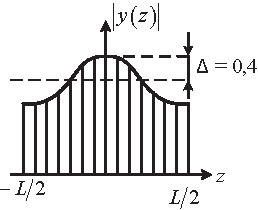
\includegraphics[width=\textwidth,height=0.35\textheight,keepaspectratio]{partial-sum-distribution}
        \caption{}%
        \label{fig:partial-sum-distribution}
    \end{subfigure}
    \begin{subfigure}[b]{0.4\textwidth}
        \centering
        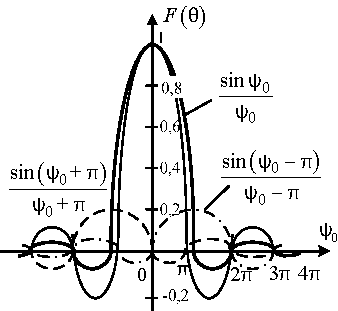
\includegraphics[width=\textwidth,height=0.35\textheight,keepaspectratio]{partial-sum-pattern}
        \caption{}%
        \label{fig:partial-sum-pattern}
    \end{subfigure}
    \caption{%
        Распределение вида “косинус на пьедестале” и соответствующая ему ДНА
    }%
    \label{fig:partial-sum-method}
\end{figure}

В зарубежной литературе классическим подходом считается применение оконных функций Дольфа-Чебышева
\cite{andreasen1962linear, harrington1961sidelobe, jain2012solving, luo2015synthesis, subbarao2015tapering, ishimaru1962theory}.

Распределение было предложено Ч. Дольфом в 1946 году \cite{dolph1946current}.
Данный метод позволяет значительно уменьшить максимальный уровень боковых
лепестков за счёт увеличения среднего УБЛ и небольшого расширения
основного лепестка. Данный способ обладает следующими преимуществами \cite{vendik2018antenna}:

\begin{enumerate}
    \item УБЛ одинаков для всех лепестков
    \item Положение боковых лепестков диаграммы направленности определяется расчётом
    \item Распределение позволяет обеспечить заданную ширину луча
\end{enumerate}

Многочлены Чебышева имеют следующий вид:

\begin{equation*}
    T_n(x)=\cos{\left[n \cdot \arccos{(x)}\right]}
\end{equation*}

Введём параметр:

\begin{equation*}
    u=\frac{2\pi d}{\lambda}\cdot \sin{\theta}
\end{equation*}

И приведём многочлены к следующему виду

\begin{equation}\label{eqn:tcheby-final}
    F(u)=\cos{\left[M\arccos{(z_0 \cdot \cos{(u\cdot z_1)})}\right]}
\end{equation}

здесь $M$ -- число элементов АР, $z_0$ -- высота и $z_1$ -- ширина главного лепестка ДНА.

Формула (\ref{eqn:tcheby-final}) определяет амплитуды.

\begin{figure}[H]
    \centering
    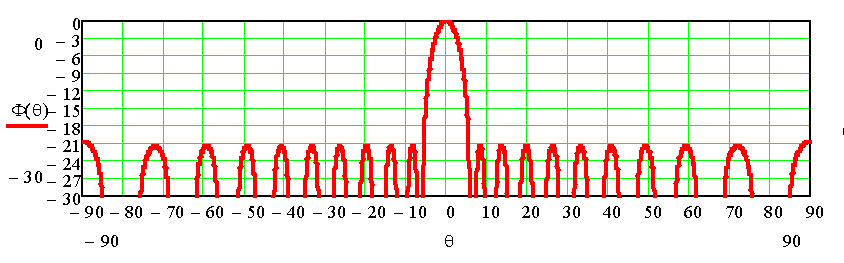
\includegraphics[width=0.8\textwidth,height=0.35\textheight,keepaspectratio]{dolph-tcheby-pattern-review}
    \caption{Диаграмма направленности антенной решётки с окном Дольфа-Чебышева \cite{vendik2018antenna}}%
    \label{fig:dolph-tcheby-pattern-review}
\end{figure}

Другими вариантами оконных функция являются также, например, оконные функции Кайзера и Блэкмана.


\subsubsection{Метод возмущений}\label{sec:perturbations-method}

Метод возмущений, представляет диаграмму направленности антенной решётки в виде суммы
парциальных диаграмм направленности, где каждый член суммы соответствует некоторому
амплитудно-фазовому распределению на элементах АР.
Сумма этих распределений даёт распределение, которое установлено в исследуемой антенной решётке.

В работе \cite{harrington1961sidelobe} рассматрено применение метода возмущений
для поиска смещений положений антенных элементов, при которых будет получена
ДНА с меньшим уровнем боковых лепестков.

Предлагается использовать расширяющееся к краям геометрическое распределение антенных элементов.
Полученное распределение сравнивается с эквидистантной решёткой с амплитудным распределением
Дольфа-Чебышёва. В Таблице \ref{table:perturbations-pos} и на Рисунке \ref{fig:perturbation-position-compare} приведены параметры антенной решётки, показанной в статье

\begin{table}[H]
    \resizebox{\textwidth}{!}{%
        \begin{tabular}{c|c|c|c|c|c|c|c|c|c|c|c|c}
            n            & 1      & 3      & 5      & 7      & 9      & 11     & 13     & 15     & 17     & 19     & 21     & 23     \\ \hline
            $\epsilon_n$ & -0,048 & -0,176 & -0,354 & -0,518 & -0,603 & -0,616 & -0,622 & -0,541 & -0,328 & +0,153 & +0,780 & +1,253 \\
        \end{tabular}
    }
    \caption{Относительные смещения элементов}\label{table:perturbations-pos}
\end{table}

\begin{figure}[H]
    \centering
    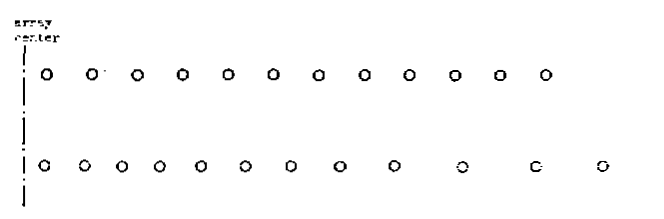
\includegraphics[width=0.8\textwidth,height=0.1\textheight,keepaspectratio]{perturbation-position-compare}
    \caption{Иллюстрация сравнения положений элементов в эквидистантной и исследуемой АР}%
    \label{fig:perturbation-position-compare}
\end{figure}

На Рисунке \ref{fig:perturbations-radial-pattern} приведены ДНА антенн исследуемой и эталонной.

\begin{figure}[H]
    \centering
    \begin{subfigure}[b]{0.4\textwidth}
        \centering
        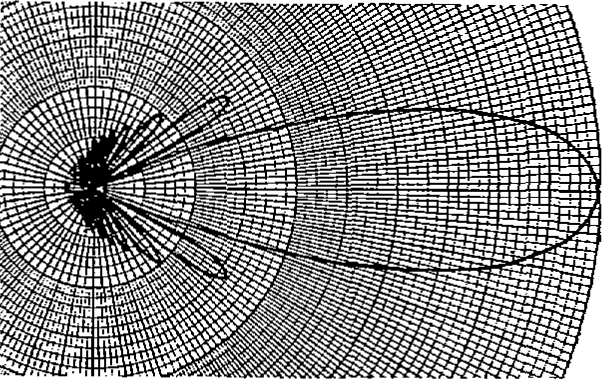
\includegraphics[width=\textwidth,height=0.35\textheight,keepaspectratio]{perturbations-radial-pattern-equidist}
        \caption{}%
    \end{subfigure}
    \begin{subfigure}[b]{0.4\textwidth}
        \centering
        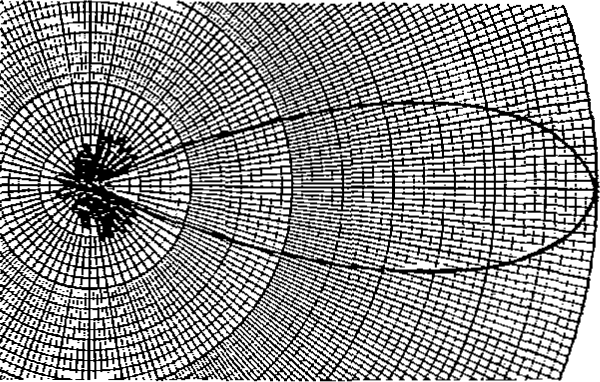
\includegraphics[width=\textwidth,height=0.35\textheight,keepaspectratio]{perturbations-radial-pattern-designed}
        \caption{}%
    \end{subfigure}
    \caption{%
        ДНА
        (а) эквидистантной и
        (б) неэквидистантной антенных решёток
        с одинаковым количеством антенных элементов.
    }%
    \label{fig:perturbations-radial-pattern}
\end{figure}

\begin{sloppypar}
    В статье, однако, отмечено, что уменьшение усиления в области ${0<u<\pi}$ ($u$ - угол от нормали к плоскости АР) приводит к
    увеличению усиления в области ${\pi<u<2\pi}$, т.е. к увеличению дифракционных лепестков, что показано на
    Рисунке~\ref{fig:perturbations-linear-pattern}. Однако это увеличение наблюдается в той области, где усиление, вызванное
    множителем решётки зачастую нивелируется уменьшением усиления множителем
    антенного элемента, что можно наблюдать на {Рисунке~\ref{fig:perturbations-radial-pattern}}.
\end{sloppypar}


\begin{figure}[H]
    \centering
    \begin{subfigure}[b]{0.4\textwidth}
        \centering
        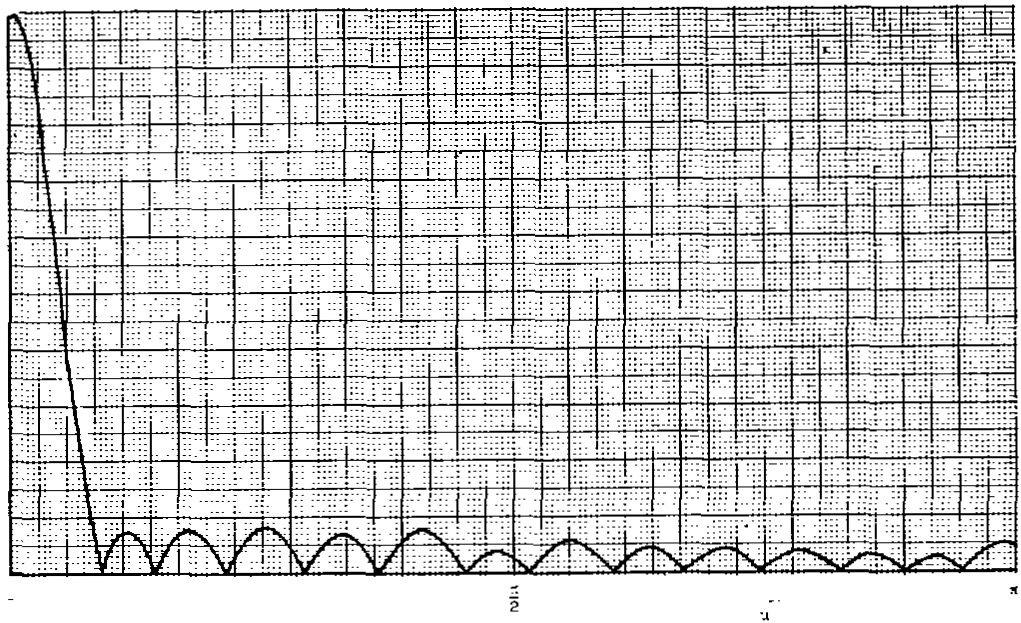
\includegraphics[width=\textwidth,height=0.35\textheight,keepaspectratio]{perturbations-linear-pattern-0pi}
        \caption{}%
    \end{subfigure}
    \begin{subfigure}[b]{0.4\textwidth}
        \centering
        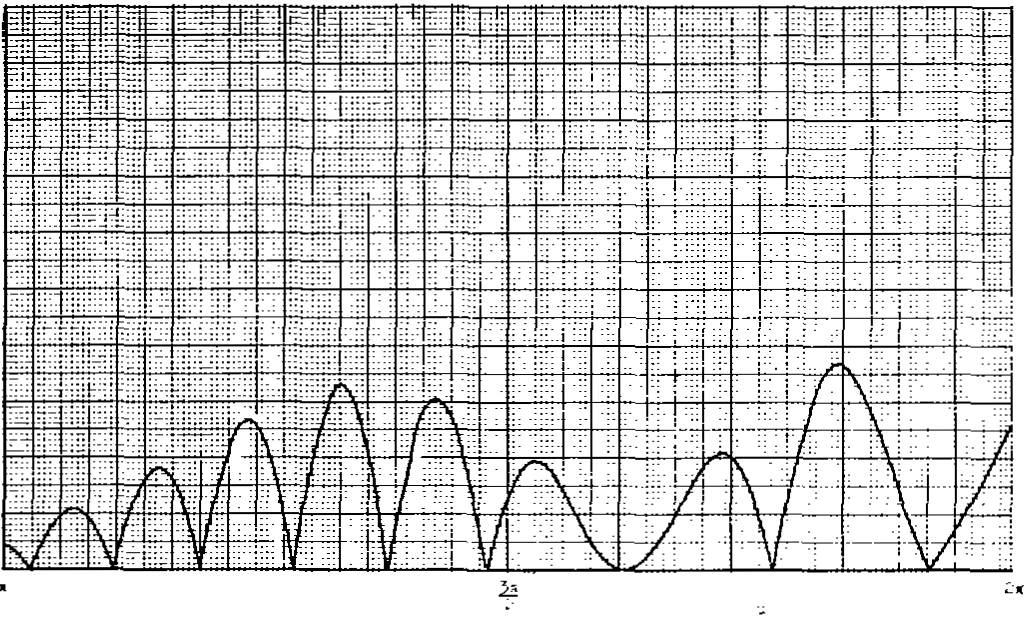
\includegraphics[width=\textwidth,height=0.35\textheight,keepaspectratio]{perturbations-linear-pattern-pi2pi}
        \caption{}%
    \end{subfigure}
    \caption{%
        ДНА при угле сканирования
        (а) от $0$ до $\pi$ и
        (б) от $\pi$ до $2\pi$
    }%
    \label{fig:perturbations-linear-pattern}
\end{figure}

Таким образом, в статье показан метод, при котором можно уменьшить УБЛ за счёт увеличения УДЛ.
При этом преимущества данного метода по сравнению с методом амплитудных распределений следующие:

\begin{itemize}
    \item не расширяется главный лепесток
    \item нет необходимости проектировать АФАР с различным усилениес в каналах, что упрощает разработку
          и удешевляет устройство
    \item больше усиление при равном количестве элементов
\end{itemize}


\subsubsection{Ряды Пуассона}\label{sec:poisson-sum}

Данный метод описан в статье \cite{ishimaru1962theory}. Здесь вводится т.н. функция положения источника,
а диаграмма направленности антенной решётки с неравномерным расположением элементов представляется в виде сумм
Пуассона ДН от множества интегральных (непрерывных) распределений элементов.
Диаграмма направленности АР описывается следующим уравнением

\begin{equation*}
    E(\theta) = \sum_{n=1}^{N} I_n e^{jks_n \sin{\theta}}
\end{equation*}

Используя формулу сумм Пуассона можно привести её к следующему виду:

\begin{equation*}
    E(\theta) = \sum_{n=-\infty}^{\infty} \int_{0}^{N} {f(\nu) e^{j2m\pi\nu} d\nu}
\end{equation*}

Далее вводится функция положения, которая связывает номер элемента с его отступом от края решётки

\begin{figure}[H]
    \centering
    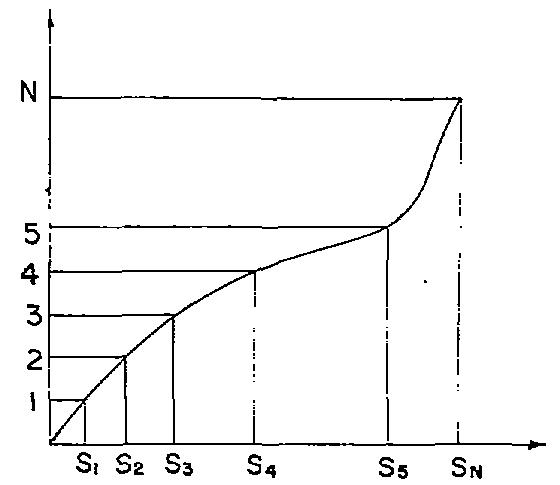
\includegraphics[width=0.8\textwidth,height=0.25\textheight,keepaspectratio]{source-position-function}
    \caption{График функции положения источника}%
    \label{fig:source-position-function}
\end{figure}

Заменив переменную перейдём к следующей формуле

\begin{equation*}
    E(\theta) = \sum_{n=-\infty}^{\infty} E_m(\theta)
\end{equation*}

\begin{equation*}
    E_m(\theta) = \int_{s_0}^{s_N} {A(s) \frac{d\nu}{ds} e^{-j(\xi(s)-2m\pi\nu(s))} e^{jks\sin\theta} ds}
\end{equation*}

Где $A(s)$ описывает амплитуду тока в решётке, причем $A(s)=A_n$ (току в $n$ элементе АР), когда $s=s_n$.

Данная сумма быстро сходится, и потому для вычисления ДН с некоторой погрешностью достаточно будет взять лишь
несколько членов этой последовательности. Так, в примере, показанном в статье, используется лишь
один член последовательности.

\begin{figure}[H]
    \centering
    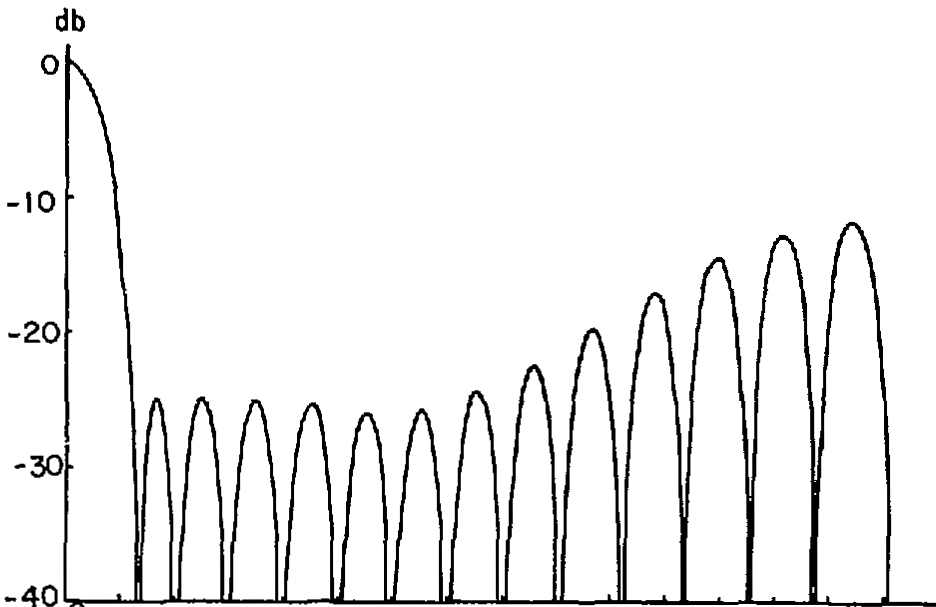
\includegraphics[width=0.8\textwidth,height=0.3\textheight,keepaspectratio]{ishimaru-20el-pattern}
    \caption{ДН антенной решётки из 20 элементов. Полученный УБЛ равен~$-25$~дБ}%
    \label{fig:ishimaru-20el-pattern}
\end{figure}

Достоинства и недостатки данного метода такие же как у метода возмущений,
рассмотренного в подразделе \ref{sec:perturbations-method}, однако распределение, полученное в статье
\cite{ishimaru1962theory}, имеет меньший уровень усиления вне главного лепестка,
чем распределение из статьи \cite{harrington1961sidelobe}.

\subsubsection{LMS алгоритм}\label{sec:lms-algorithm}

В статье "Weighted Least Square method for Optimum Thinned Antenna Arrays" авторы Xinyu Ma и Byong Kun Chang
рассматривают проблему оптимизации антенных решёток, используя взвешенный метод наименьших квадратов. Основная
задача, решаемая в статье, заключается в нахождении оптимальных межэлементных расстояний в разреженных (thinned)
антенных решётках для получения желаемых характеристик при заданном количестве элементов.

Процесс нахождения наиболее подходящих межэлементных расстояний следующий:
\begin{sloppypar}
    \begin{enumerate}
        \item Определение функции ошибки

              $$
                  E^k (\omega) = W(\omega)\left[H_d(\omega)-H_l^k (\omega)\right]
              $$

              здесь $H_l^k$ -- ДН на k-той итерации, $H_d$ -- эталонная ДН, а $W(\omega)$ -- взвешивающая функция.

              Тогда итоговая ошибка рассчитывается как интегральных

              $$
                  \epsilon^k = \frac{1}{2} \int_{0}^{\pi}{ \left| E^k(\omega) \right|^2 d\omega}
              $$

        \item Итеративное обновление параметров

              Ошибка $\epsilon^k$ может быть аппроксимирована как квадратичная функция от изменений межэлементных расстояний
              $\Delta D_n$. На каждом шаге изменение расстояний рассчитывается как

              $$
                  \Delta D_{n}^{k+1}-\mu \frac{\partial \epsilon^k}{\partial \Delta D_n^k},\ 1\leq n \leq N_l
              $$

              здесь $\mu$--шаг сходимости ДЬЫ алгоритма, $\Delta D_n^k$ и $\Delta D_n^{k+1}$ -- изменения межэлементных расстояний на {k-том} и {k+1-ом} шаге алгоритма, а $\frac{\partial \epsilon^k}{\partial \Delta D_n^k}$~--~градиент-вектор квадрата ошибки.

              Межэлементное расстояние получается как

              $$
                  D_{n}^{k+1} = \Delta D_{n}^{k} + \Delta D_{n}^{k+1}, \ 1\leq n \leq N_l - 1
              $$

    \end{enumerate}
\end{sloppypar}

Функция взвешивания определяется следующим образом

\begin{equation*}
    W(\omega) =
    \begin{cases}
        1 & \text{$\omega\in [0, \omega_p]$}    \\
        c & \text{$\omega \in [\omega_p, \pi]$}
    \end{cases}
\end{equation*}

\noindent здесь $\omega_p$ -- половина ширины главного лепестка диаграммы направленности, а $c$ -- некоторая константа.

Таким образом можно регулировать насколько важны параметры УБЛ и ширины главного лепестка. 
В статье принимают $c>1$, таким образом повышая приоритет требования по уровню боковых лепестков. 
Одним из вариантов $W(\omega)$ в статье является функция экспоненциального взвешивания:

\begin{align*}
    & W(\omega) =
    \begin{cases}
        1 & \text{$\omega\in [-\omega_p, \omega_p]$}    \\
        Be^{-A(\omega-\omega_p)} & \text{$\omega \in [\omega_p, pi]$}    \\
        Be^{A(\omega-\omega_p)} & \text{$\omega \in [-\pi, \omega_p]$}
    \end{cases}
\end{align*}

\noindent здесь $A$ и $B$ -- константы, контроллирующие параметры экспоненциального взвешивания.

Результаты работы алгоритма показаны на Рисунках~\ref{fig:lms-101-dolph}~-~\ref{fig:lms-51-learning-curve}.

\begin{figure}[H]
    \centering
    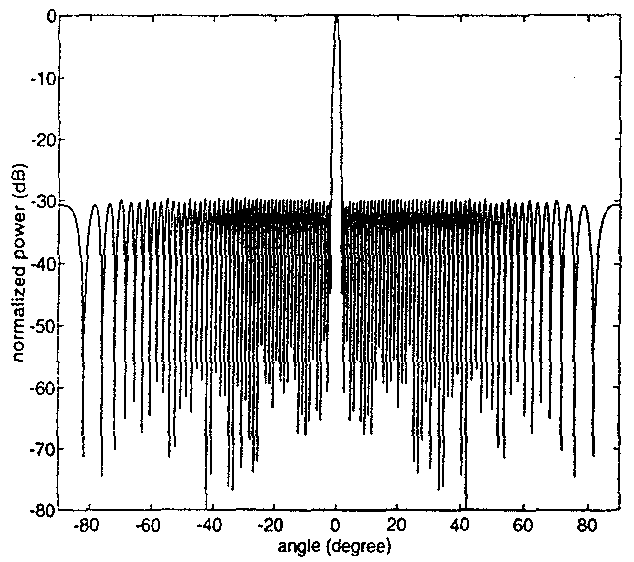
\includegraphics[width=0.8\textwidth,height=0.25\textheight,keepaspectratio]{lms-101-dolph}
    \caption{ДН эталонной решётки из 101 элемента, синтезированной методом Дольфа-Чебышёва}%
    \label{fig:lms-101-dolph}
\end{figure}

\begin{figure}[H]
    \centering
    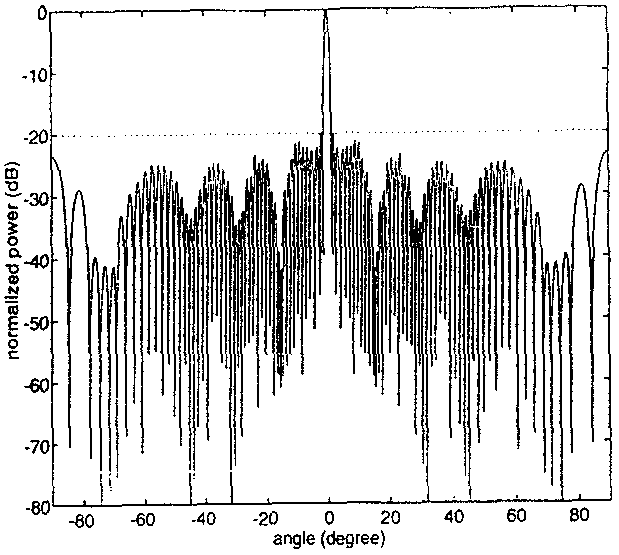
\includegraphics[width=0.8\textwidth,height=0.25\textheight,keepaspectratio]{lms-51-rp}
    \caption{Диаграмма направленности АР из 51 антенного элемента, оптимизированной LMS алгоритмом}%
    \label{fig:lms-51-rp}
\end{figure}

\begin{figure}[H]
    \centering
    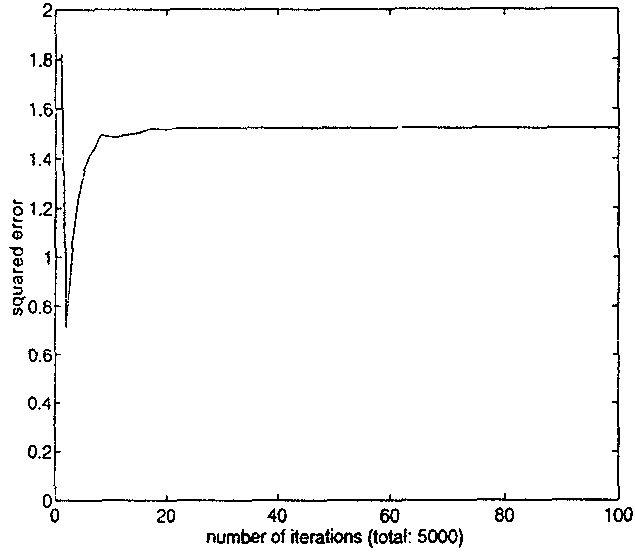
\includegraphics[width=0.8\textwidth,height=0.25\textheight,keepaspectratio]{lms-51-learning-curve}
    \caption{ Кривая обучения LMS алгоритма}%
    \label{fig:lms-51-learning-curve}
\end{figure}




\subsubsection{Вероятностные методы}\label{sec:stochastic-algorithms}

Предыдущие подразделы описывали различные методы нахождения оптимальных распределений с использованием математических 
методов и функций оптимизации. Методы, описанные в данном подразделе, используют различные эволюционные алгоритмы 
для нахождения оптимальных распределений.

Проблема нахождения оптимальных распределений часто рассматривается как комбинаторная задача. Однако с увеличением 
размеров антенных решёток, количество вычислений растёт экспоненциально. \cite{jain2012solving}. Так как вычислительные методы 
с трудом применимы для разреживания больших антенных решёток, на помощь приходят вероятностные методы. Данная группа 
методов включает в себя генетические алгоритмы, муравьиные (ant colony algorithm) и 
кошачьи (cat swarm optimization) алгоритмы, метод роя частиц (particle swarm optimization), 
алгоритм классной комнаты (Teaching-learning-based optimization) и другие. 

Задача оптимизации антенной решётки с точки зрения комбинаторики является дискретной, комбинаторной и NP полной, что 
означает, что время расчёта значительно возрастает при использовании классических методов. В то же время стохастические 
методы позволяют более эффективно решать проблемы приближенного поиска глобального максимума или минимума во 
всё возрастающем пространстве решений. 

В качестве примера рассмотрим алгоритмы, описанные в \cite{jain2012solving} и \cite{luo2015synthesis}. 

Основы эволюционных алгоритмов следующие:
\begin{itemize}
    \item Популяция в генетических алгоритмах состоит из множества решений, представленных уникальными “хромосомами”. 
    Хромосома -- это закодированная строка, в которой каждый символ представляет один параметр решения
    \item Каждый индивидуум (каждое решение) оценивается на основе некоторой функции пригодности, которая сравнивает 
    полученное решение с другими и с эталонными
    \item На основе результатов функции селекции (пригодности) выбираются решения для создания следующего поколения через 
    генетические операции, такие как мутация и кроссовер. Кроссовер -- генетический оператор, который создаёт потомство как 
    комбинацию параметров двух родителей. Мутация -- случайное изменение в параметрах отдельных хромосом. Мутация нужна для 
    избежания локальных экстремумов и поддержания генетического разнообразия в пространстве решений.
\end{itemize}

В работах \cite{jain2012solving} и \cite{luo2015synthesis} генетические алгоритмы применяются следующим образом:

\begin{itemize}
    \item Алгоритм применяется к изначально созданному равномерному распределению на плоском раскрыве. Рассматриваются 
    прямоугольная и круглая решётки соответветственно. 
    \item На каждом шаге алгоритм отключает и включает отдельные элементы решётки
    \item У каждого элемента всего 2 состояния, таким образом каждый ген хромосомы кодируется одним битом и может
    принимать значения либо 0 либо 1.
\end{itemize}


\begin{figure}[H]
    \centering
    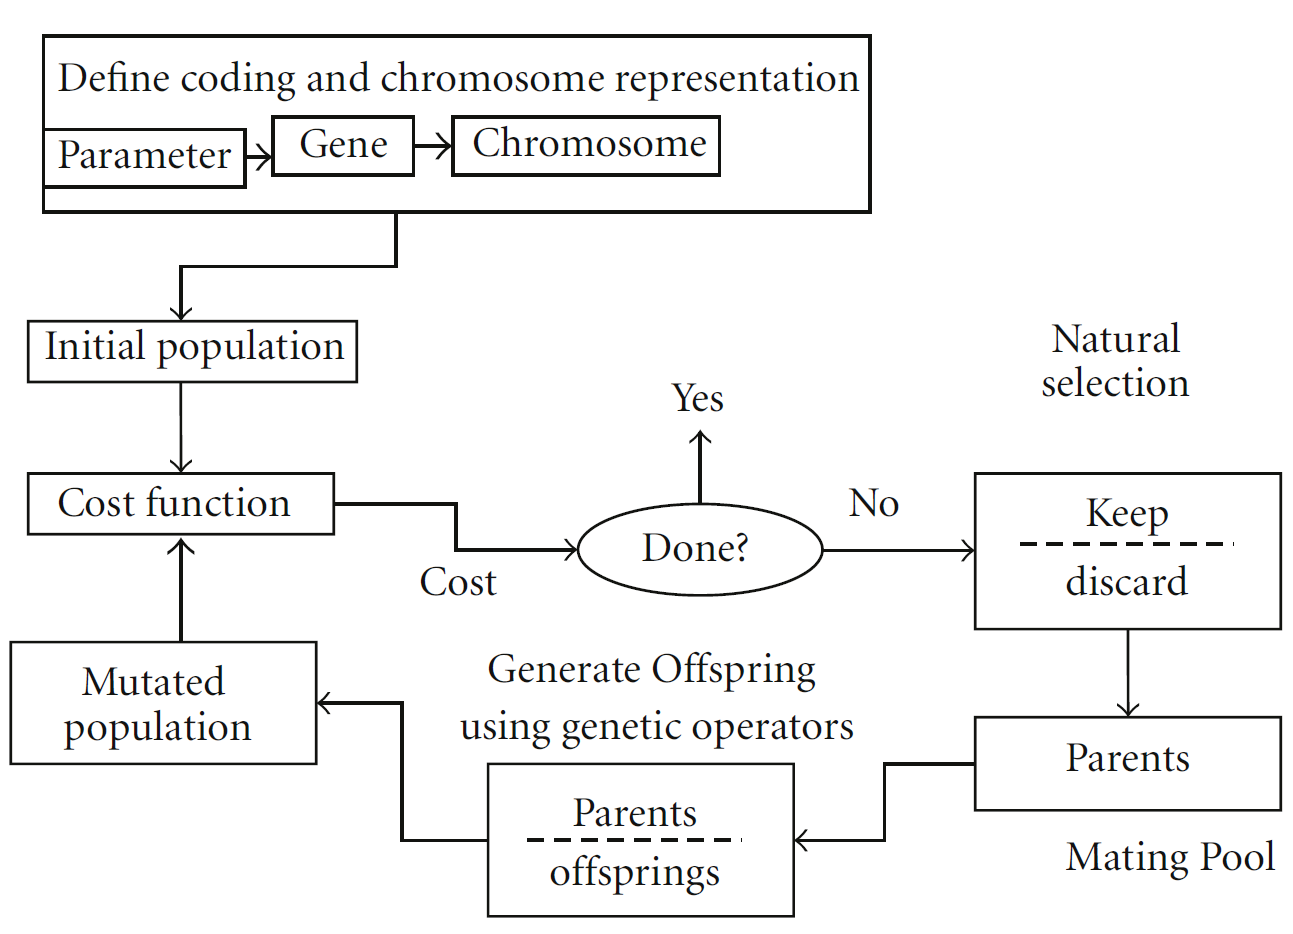
\includegraphics[width=0.8\textwidth,height=0.3\textheight,keepaspectratio]{genetic-algorithm-explanation}
    \caption{Блок-схема простейшего генетического алгоритма}%
    \label{fig:genetic-algorithm-explanation}
\end{figure}

На Рисунках~\ref{fig:genetic-algorithm-pattern-3060}-\ref{fig:genetic-algorithm-pattern-6000} показаны результаты работы ГА для разных направлений прихода сигнала.

\begin{figure}[H]
    \centering
    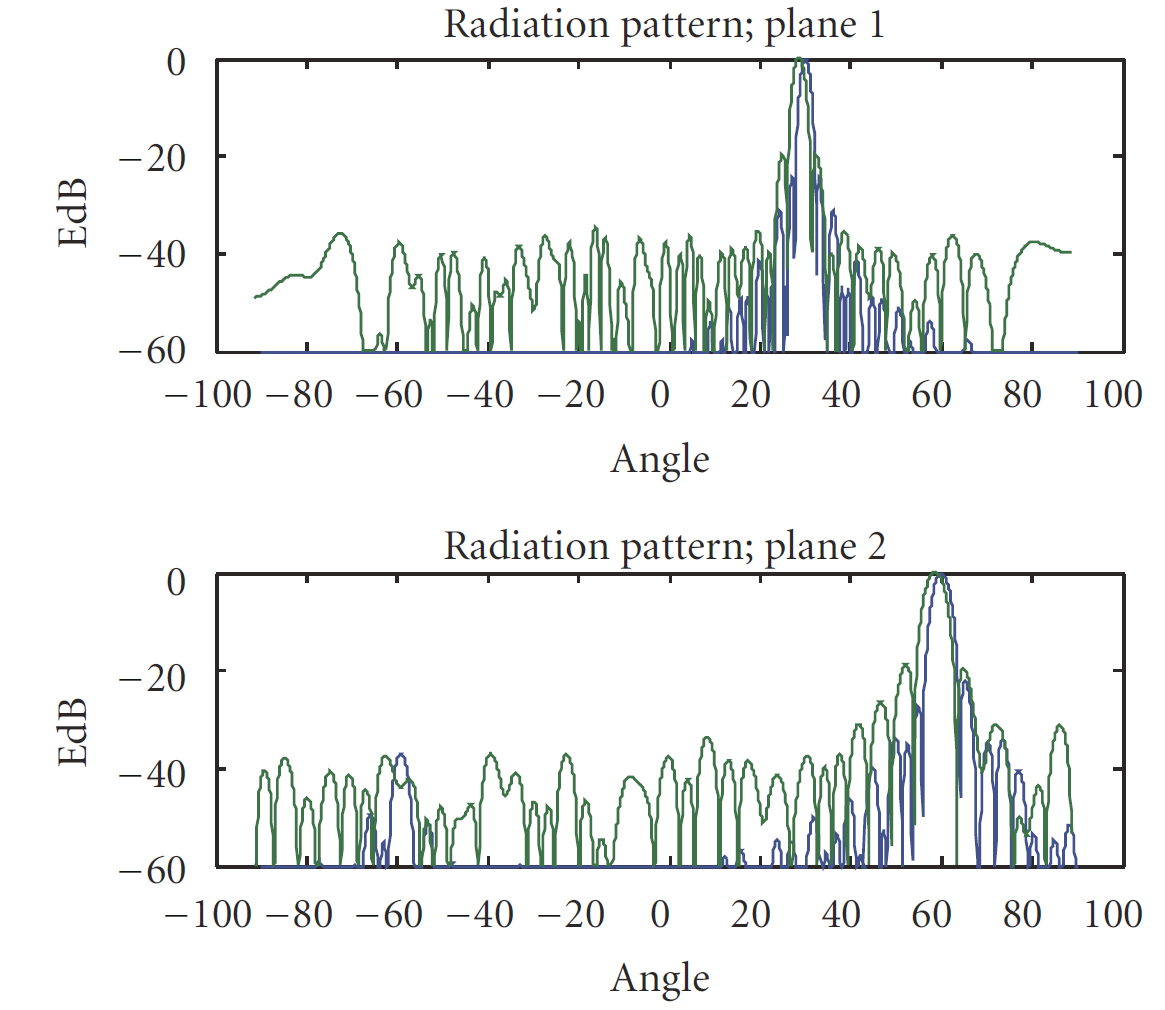
\includegraphics[width=0.8\textwidth,height=0.35\textheight,keepaspectratio]{genetic-algorithm-pattern-3060}
    \caption{ДНА полученной АР в направлении $\theta=30$, $\phi=60$}%
    \label{fig:genetic-algorithm-pattern-3060}
\end{figure}


\begin{figure}[H]
    \centering
    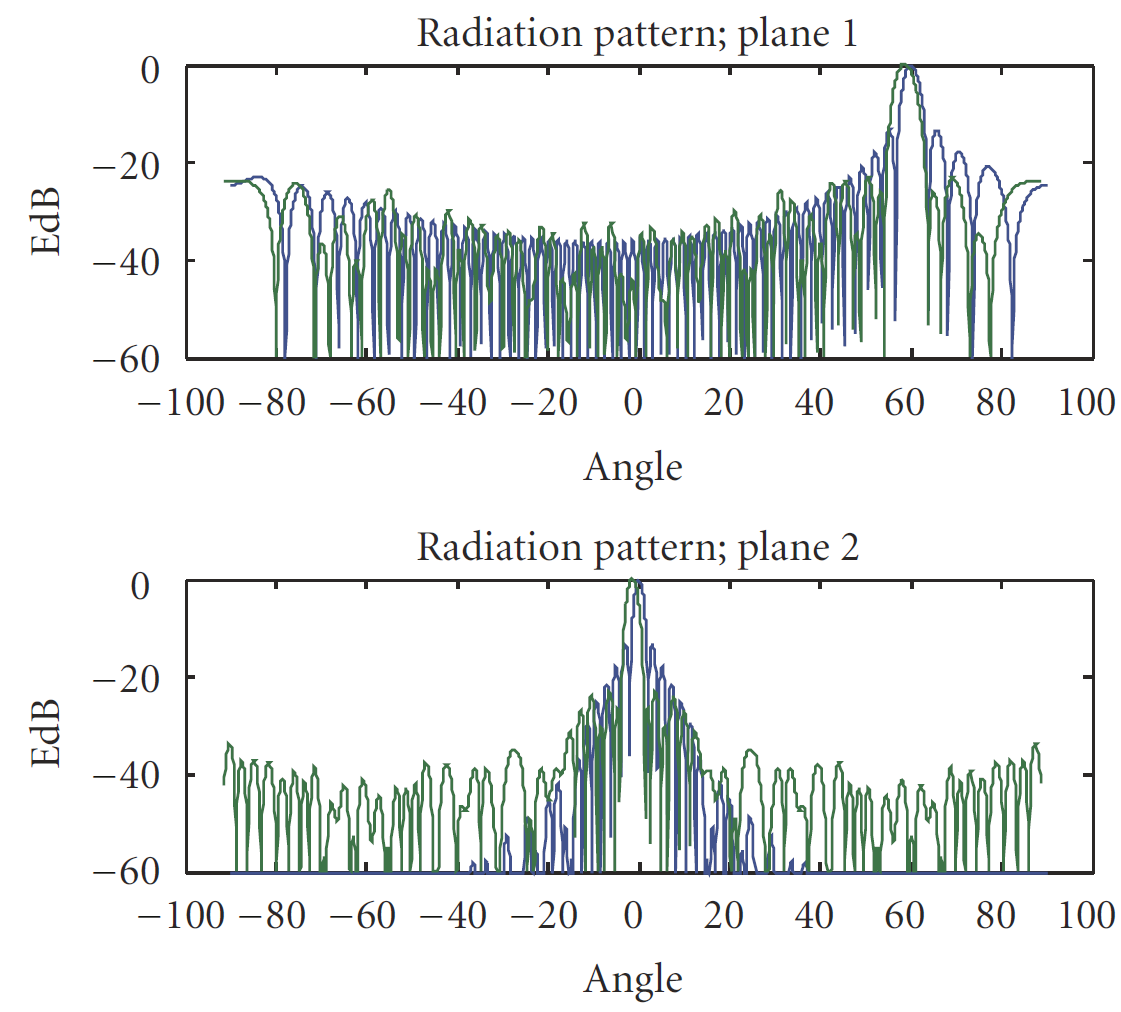
\includegraphics[width=0.8\textwidth,height=0.35\textheight,keepaspectratio]{genetic-algorithm-pattern-6000}
    \caption{ДНА полученной АР в направлении $\theta=60$, $\phi=0$}%
    \label{fig:genetic-algorithm-pattern-6000}
\end{figure}
